\chapter{Additions to the evaluation}\label{chpt:evaluationAdditions}
\glsresetall

\section{Training metrics}\label{sec:ea:trainingMetrics}

\begin{table}[H]
	\centering
	\captionabove[Overview of all metric results.]{Overview of metric results for different training tasks and data splits.}
	\label{tab:ea:metricResults}
	\begin{tabular}{p{0.03\textwidth}p{0.17\textwidth}p{0.03\textwidth}p{0.14\textwidth}p{0.03\textwidth}S[table-format=1.3]S[table-format=1.3]S[table-format=1.3]S[table-format=1.4]}
		\toprule
		&  \multicolumn{1}{c}{Training task} &&  \multicolumn{1}{c}{Epoch} && \multicolumn{1}{c}{$P$} & \multicolumn{1}{c}{$R$} & \multicolumn{1}{c}{$mAP_{50}$} & \multicolumn{1}{c}{$mAP_{50-95}$} \\
		\midrule
		%
		\multicolumn{9}{l}{\bfseries{Model 1, Validation data}} \\[7pt]
		%
		&  \multicolumn{1}{c}{\textsc{train}} &&  \multicolumn{1}{c}{\textsc{best}} && 0.982 & 0.974 & 0.988 & 0.664 \\[5pt]
		&  \multicolumn{1}{c}{\textsc{finetune}} &&  \multicolumn{1}{c}{\textsc{best}} && 0.993 & 0.988 & 0.995 & 0.825 \\[7pt]
		%
		\multicolumn{9}{l}{\bfseries{Model 1, Test data}} \\[7pt]
		%
		&  \multicolumn{1}{c}{\textsc{train}} &&  \multicolumn{1}{c}{\textsc{best}} && 0.974 & 0.977 & 0.991 & 0.661 \\[5pt]
		&  \multicolumn{1}{c}{\textsc{finetune}} &&  \multicolumn{1}{c}{\textsc{best}} && 0.981 & 0.991 & 0.994 & 0.819 \\[7pt]
		%
		\multicolumn{9}{l}{\bfseries{Model 2, Validation data}} \\[7pt]
		%
		&  \multicolumn{1}{c}{\textsc{train}} &&  \multicolumn{1}{c}{\textsc{best}} && 0.985 & 0.992 & 0.993 & 0.682 \\[7pt]
		%
		\multicolumn{9}{l}{\bfseries{Model 2, Test data}} \\[7pt]
		%
		&  \multicolumn{1}{c}{\textsc{train}} &&  \multicolumn{1}{c}{\textsc{best}} &&  0.983 & 0.99  & 0.991 & 0.676 \\
		%
		\bottomrule
	\end{tabular}
\end{table}

\newpage

\section{Inference results}\label{sec:ea:inferenceResults}

\begin{figure}[H]
	\centering
	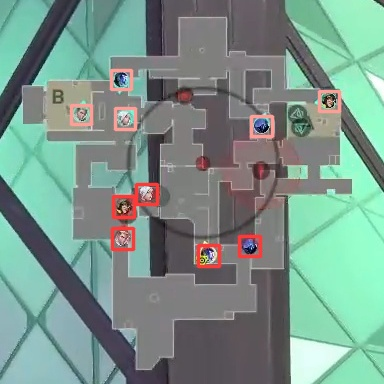
\includegraphics[width=0.8\linewidth]{images/a02-detect}
	\caption[Detected bounding boxes.]{Detected bounding boxes for a not trained image from the map "Ascent".}
	\label{fig:ea:outDetect}
\end{figure}

\begin{figure}[H]
	\centering
	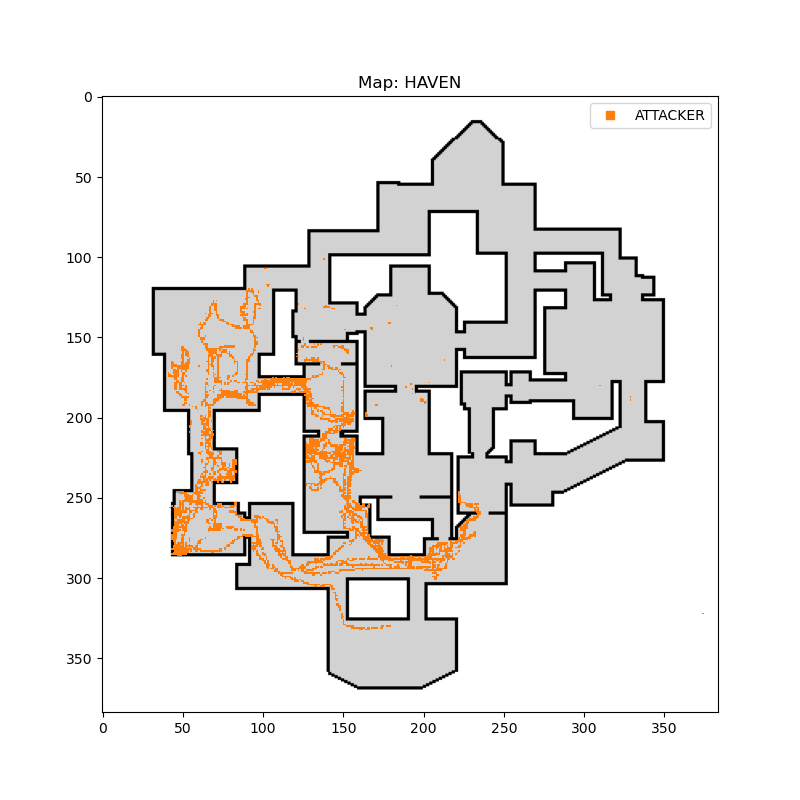
\includegraphics[width=0.95\linewidth]{images/a03-att-output}
	\caption[Output representation as map for attacker.]{Output representation as map, summarizing all positions 
		of attacker agents during one round on the map "Haven".}
	\label{fig:ea:outputAtt}
\end{figure}

\begin{figure}[H]
	\centering
	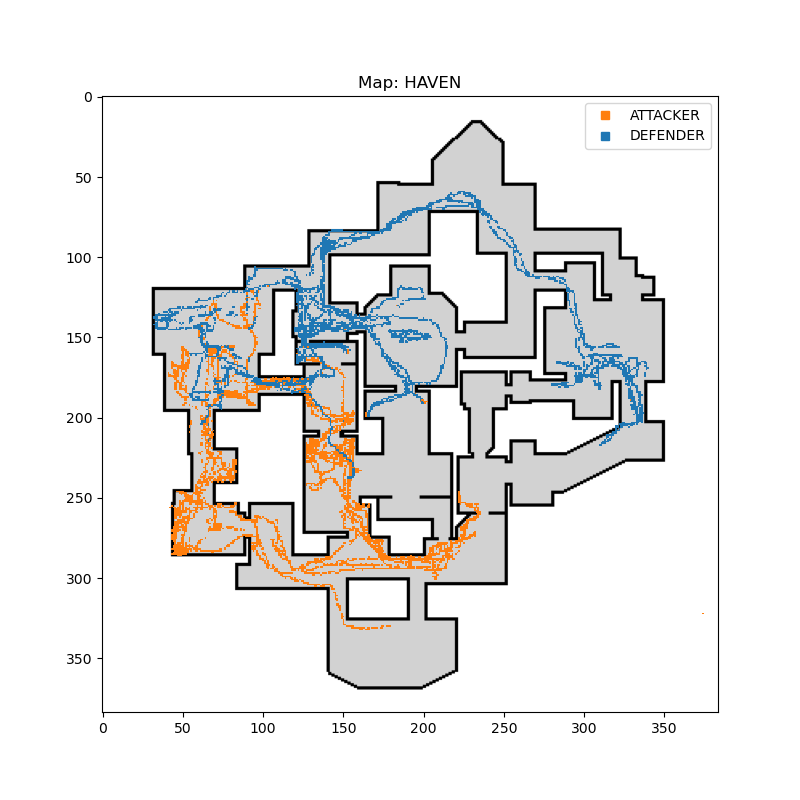
\includegraphics[width=0.95\linewidth]{images/a04-comb-output}
	\caption[Output representation as map.]{Output representation as map, summarizing all positions 
		of defender and attacker agents during one round on the map "Haven".}
	\label{fig:ea:outputComb}
\end{figure}